%% Aggregate text that works for the theory here:

\chapter{A Personnel Resource Curse}
\label{chapter:theory}
%Chapter introduction:

%% The intro is actually different: this talks about why there might be rapid expansion. But the model is actually about the negotiation model.

%% Really I need accommodation model, which creates the personnel resource curse. Because of the negotiation/accommodation model of management, then recruitment puzzle. Without the negotiation/accommodation model, growth would not be so puzzling. Instead, growth would be a straightforward advantage for the leader: more people, more capacity.

This chapter focuses on the negotiation step of the leader-subordinate relationship, and highlights how needing buy-in results in a leader who accommodates the preferences of their base. It presents a model of leader accommodation, with a particular focus on the effect of incomplete socialization and labor mobility on the ability of the base of an organization to demand strategic and directional change. 

The model frames negotiation and bargaining as at the center of the relationship between a leader and their rank and file. Leaders who maintain strong leverage positions— such as by being able to use financial tools, threats of violence, or threats of termination — are more able to delegate their preferred activities and monitor compliance from their personnel.  However, not all leaders have a strong enough position to be able to accomplish this. In particular, as the model highlights, highly desirable recruits may also be those that are most difficult to socialize.

%% Here explain why I'm claiming to present a project about recruitment shocks and bottom-up organizational change, but first talking about within-organization decisions 
To connect recruitment shocks to downstream organizational changes, the chapter introduces the negotiation mechanism that drives the process of accommodation and transformation. The mechanism expects that recruitment shocks will promote changes in organizational focus and strategy, even against the preferences of the original leadership. After presenting the theory in general, I analyze the implications of the model, with particular emphasis on predicting when observers should expect an organization to undergo bottom-up internal transformation.


\section{Negotiation Framework}

I present a formal model of the transformation mechanism by which a leader incrementally adjusts the mission of their organization to reflect the interests and goals of their rank-and-file. The model describes a strategic game between leaders and recruits, emphasizing the intuition of the game and equilibrium expectations.

By representing the internal dynamics of activity generation through a  model of negotiation in which the subordinates accept or reject an action proposed by the leader, the model formalizes a pervasive, but largely implicit conceptualization of the limits of hierarchy in organizations.  The intuition that subordinate buy-in is important for the smooth operation of organizations can be seen in the large literature on the benefits of democratic and consensus-based management styles (\textit{e.g}~\cite{covin1988influence, kastelle2013hierarchy, morris2000experimental}) and, conversely, in research into the effect of employee (dis)engagement on destructive and non-compliant behaviors (\textit{e.g.}~\cite{ariani2013relationship,dalal2012relative, spector2010counterproductive}). Finally, the vast popular management literature advising practitioners on how to obtain employee or subordinate \say{buy-in} for initiatives also reinforces the intuition that a negotiation model captures a fundamental insight into the dynamics of within-organizational operations~(\textit{e.g}~\cite{broder2013buy, hedges2015buy,hubspot2020tips, kotter2010buy, ridzi2004making, thomson1999buy, thomson2000business}).

\subsection{Accommodation Model}
%Here explain why the model is structured as a bargaining model:

The basic setup of the model is that a Leader is presented with an opportunity to recruit new members whose preferences may or may not align with the preferences of the leader. The Leader and the prospective Recruit[s both know that after entering into the organization, the recruit will experience some degree of socialization--via training, indoctrination, or other activity--that will shift their preferences. However, neither the leader nor the recruit can predict the extent to which the recruit’s preferences will align with those of the leader. Once the recruits have been incorporated into the bulk of the organization, the organization can only act if both the leader and the recruits agree on an activity. 

\subsection{Game}

The model has two actors: the Leader (L) and the Recruit (R). The Recruit represents some subset of a larger population of potential supporters. The subset that is available to the leader to recruit from is a random draw from a larger pool of potential supporters. For clarity, the Recruit is referred to in the singular because the Recruit's decisions, socialization, and goals are represented as unitary. Likewise, for simplicity, the model treats the \say{Leader} as a single actor that behaves as it if has unitary preferences.\footnote{This elides the reality that in many organizations, leaders have diverging preferences and -- sometimes bitter-- disputes over which preferences will be used to set organizational priorities. The model treats the resolution of this competition as exogenous in favor of focusing on the leader-recruit negotiation over preferences. }

The game begins after the Leader has seen the random draw from the recruitable population. This random draw furnishes the Recruit (R) in the game. The Leader must weigh whether or not to try to incorporate the potential Recruit into the organization, while the Recruit decides whether to accept.  The Leader is incentivized to try to grow via recruitment, because the new Recruit brings the resources needed for continued operation. Correspondingly, the Recruit is motivated to join both by the potential benefits of a successful operation as well as a private value for belonging to an organization.

The sequence of play can be seen in Figure~\ref{fig:rg}, and proceeds as follows: In the first stage, the Leader, who has goals $G_{L}$, interviews the potential recruits that they have selected. The Recruit(s) has an initial goal $G^{0}_{R}$, which the interview reveals to the Leader. If the interview indicates that the Recruit's resource level and goals are acceptable, the Leader can choose whether or not to offer membership. The Leader pays the interview cost $C_{I}$ regardless of whether or not the Recruit accepts, as this represents the cost to evaluating potential recruits.
The Recruit can then accept or reject this offer, incurring a penalty of $-U_{G}$ if they decline the offer.  $U_{G}$, which is explored in more depth in the game analysis, represents a private utility that the Recruit gains for being part of an organization. $U_{G}$ can be either material (such as wages or access to goods and services) or immaterial (such as by generating social connections or bolstering a self-identity). In either case, the term represents the value that the Recruit derives from membership.

\begin{center}
  \begin{figure}
    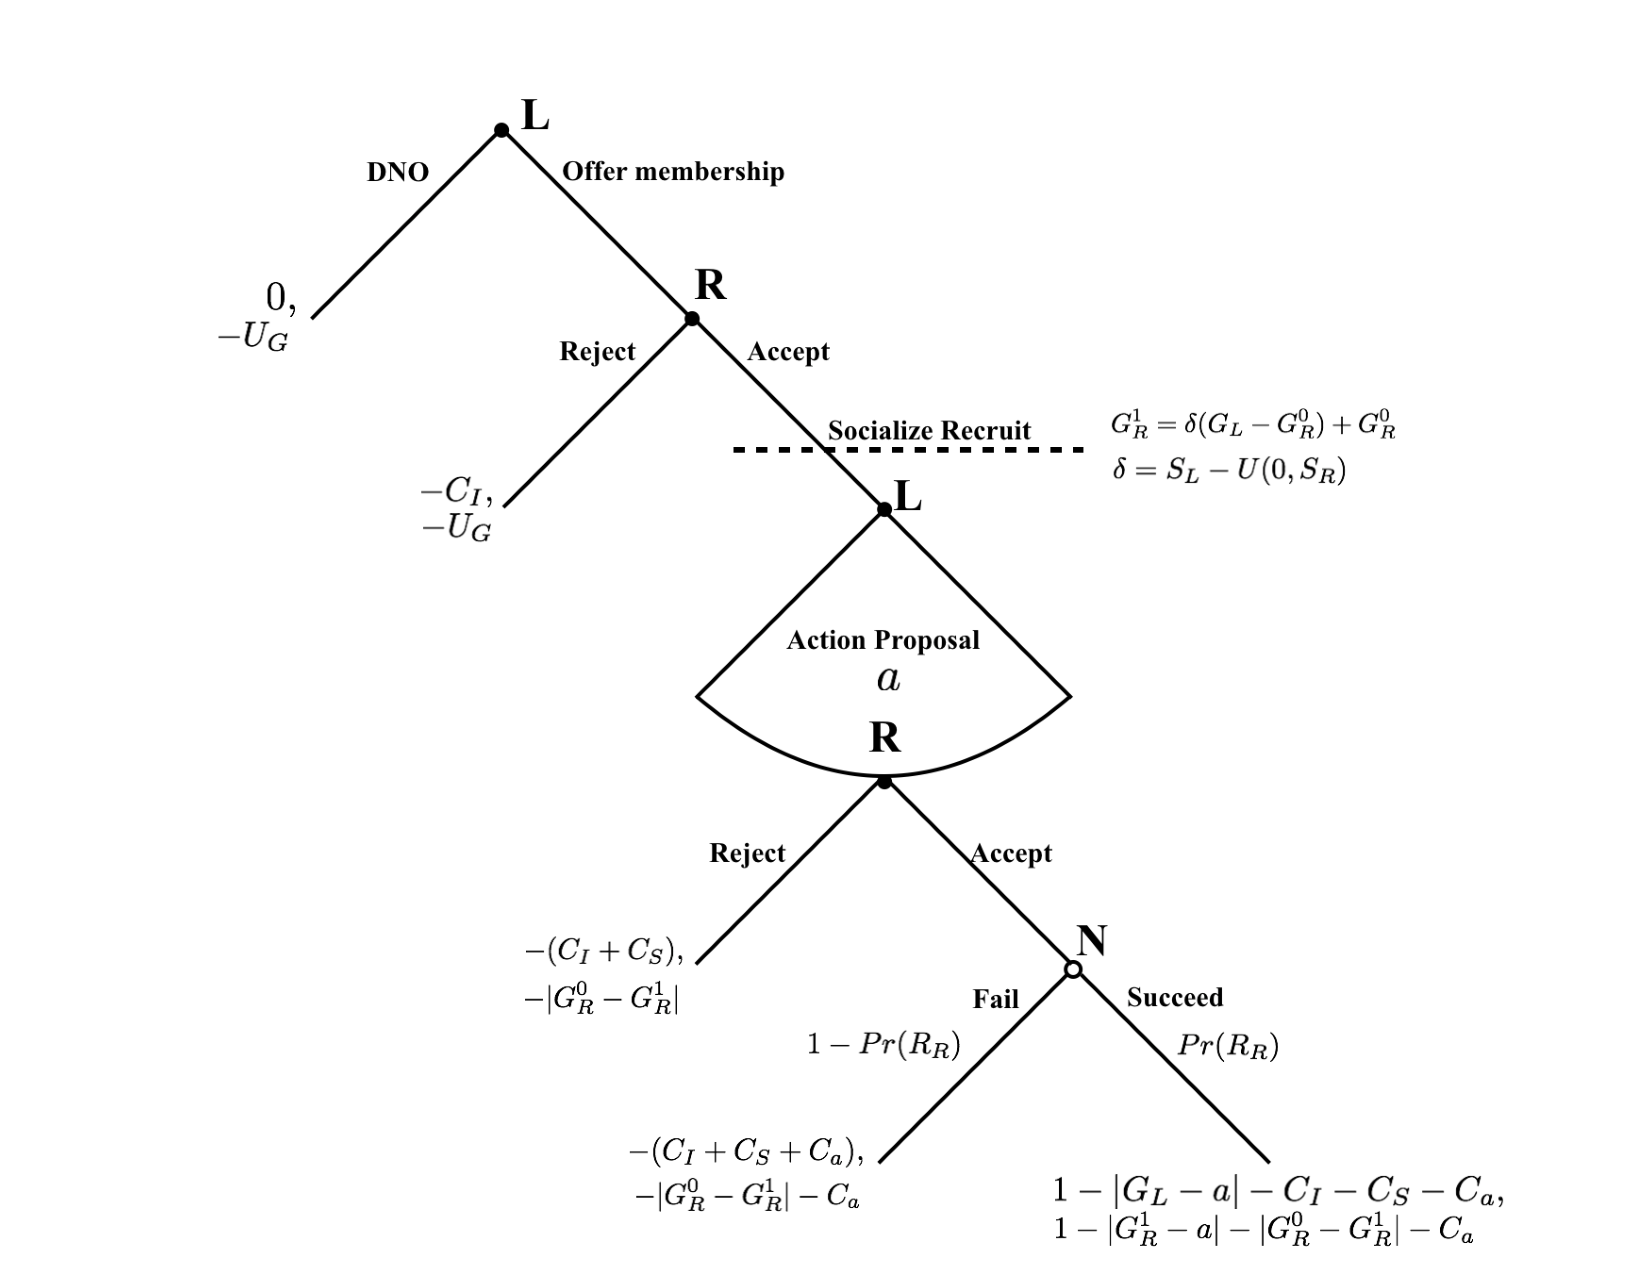
\includegraphics[width=\columnwidth]{./Pictures/RecruitGame_Round1.pdf}
    \caption{Single Round Recruitment Game Tree}
        \label{fig:rg}
     \end{figure}
\end{center}

If the Recruit accepts the membership invitation and joins the organization, they contribute their resources ($R_{R}$) to the group and undergo some level of socialization that brings their goals more into alignment with the Leader's original goals. After this socialization period, the goals of the recruit become $G^{1}_{R}=\delta(G_{L}-G^{0}_{R}) + G^{0}_{R}$ where $\delta$ represents the Leader's socialization capacity.

The socialization process is parameterized by: $\delta \sim f(S_{L}, S_{R})$. Modeling socialization as a function of Leader capacity and Recruit capacity allows the model to incorporate contextually-specific features of the recruitable population, the leader's resources, or the group's needs that may influence socialization. For example, a dense social network among a subset of the recruitable population would make that portion of the recruiting space more challenging to socialize (and thereby represent a larger value of $S_{R}$, leading, in expectation, to a lower value of $\delta$ for those recruits). Conversely, features that enhance the socialization capacity of the Leader---such as an ideological curriculum or training camps---increase the value of $\delta$. The Leader's socialization capacity, which is analyzed at greater length in the subsequent section, captures the average ability of the Leader $S_{L}$ to tilt the recruit's original goals ($G^{0}_{R}$) towards the goals of the Leader ($G_{L}$).  During the socializing process, the Leader's ability to align $G^{1}_{R}$ with $G_{L} $ mitigated by the ability of the recruit to retain their original preferences ($S_{R}$).\footnote{Because the difficulty of socialization is a random variable neither the Leader nor the prospective recruits can predict the exact degree to which socialization will be successful. Therefore, both the Leader and the Recruits use the expected value of the socialization round in maximizing their utility.  Modeling the difficulty of socializing new recruits as a random variable introduces flexibility in the model that allows it to model an array of contexts.} Socialization shifts the recruit's goals to $G^{1}_{R}$ and entails socialization cost $C_{S}$ from the Leader. 
 
For simplicity, the solution presented here assumes that the difficulty of socialization is distributed uniformly throughout the population of potential recruits, and so, $\delta \sim$ Unif$(0, S_{L}- $Unif$[0, S_ {R}])$.\footnote{Equivalently, $\delta$ can be conceptualized as a Beta distribution with hyperparameters $\alpha = \beta = 1$. This parameterization is equivalent to the Uniform distribution presented here, but would allow for a Bayesian interpretation of the socialization parameter.} Thus, for both the leader and the recruits, the expected socialization is $E(\delta) = \frac{1}{2}(S_{L} + \frac{1}{2}(S_{R}))$.  The post-socialization goals of the recruit are given as: $G^{1}_{R} = \delta(G_{L}-G^{0}_{R})+ G^{0}_{R}$. In effect, the Recruit's goals after socialization represent a linear combination of the Leader's goals and the Recruit's initial goals, weighted by a socialization capacity.

After the socialization stage, the Leader chooses whether to propose an activity ($a$) to the Recruit. The objective of the activity lies on some span between the goal of the Leader and the updated goal of the Recruit. The activity proposal occurs after the socialization, at which point the Leader and the Recruit jointly know the extent to which the Recruit's updated goal has converged with the Leader's goal. 

After observing the proposed activity $a$, the Recruit decides whether or not to accept the action. If they reject the offer, their resources are withdrawn from the group, but the Recruit retains the post-socialization goal. The Leader loses all overhead from identifying and socializing the recruits.  If the Recruit accepts, the action succeeds or fails with a probability based on the resources brought to bear on the action. 

The resources that can be applied to the action consist of the resources that the Recruit brings to the organization ($R_{R})$.  If the activity is successful, both the Leader and the Recruit derive utility proportional to the distance between the activity and their ideal goals. If the activity is unsuccessful, the Leader and the Recruit each lose the resources they have invested. Moreover, the Recruit takes a penalty to their utility proportional to the distance between their original goals and their post-socialization goals.  This socialization penalty is not borne by Recruit after a successful action.\footnote{This assumption can be considered as a utility boost from being part of a successful organization.}

At the conclusion of the first round of activity, the Leader's goals update to be a weighted linear combination of the Leader's original goal and the successful activity. Thus, the Leader's updated goal is $G^{1}_{L}= \alpha(G^{0}_{L}) +(1-\alpha)a$. Updating the Leader's goals allows their objectives, and the objectives of their group, to vary according to the activities the group successfully carries out.\footnote{This updating does not necessarily have to represent the Leader internalizing the new activities that the group has been engaging in. It could also represent the influence of personnel changes rising through the ranks of the organization. In this case, the \say{Leader} role is unitary, and so emerging heterogeneity in the preferences of a leadership corps is represented in a single Leader goal.} 

After the Leader's goals update, the game enters another round, with the Leader seeking a new set of Recruits.  However, the Leader begins the round from the new starting point of $G^{1}_{L}$.  

\subsection{Equilibrium Expectations}

In theory, a perfectly rational leader can infinitely look down the game tree and generate expected values of the distribution of ideal points in the recruitment pool and the expected level of socialization that they will be able to apply. However, in reality, predictions increase in uncertainty the further out they are applied. In order to capture the uncertainty of real-world decision making and continued operation of any given organization, the equilibrium presented in the following section truncates the model after two rounds.

In equilibrium, Leader knows how successfully the Recruit has been socialized and should select a proposed activity $a$ that minimizes the distance between the proposed activity and the Leader's goal and the proposed activity and the Recruit's post-socialization goal. A leader with a larger value of $S_{L}$ should be more successful in socializing and should consequentially produce a post-socialization Recruit goal that is closer to the original goal of the Leader. Consequentially, these high-capacity leaders should propose actions $a$ that are located closer to the Leader's original goal.  

Conversely, a Leader with a weaker capacity for socialization should be incentivized to propose an action that is closer to the Recruit's preferences. A weak Leader faces an upstream choice about whether or not to recruit. If they decide not to recruit, the weak Leader will be unable to field activities while still maintaining the overhead costs of interviewing potential recruits. On the other hand, they can choose to recruit new members who have resources but who the Leader will not expect to be able to completely socialize. This will require the Leader to propose actions that are further from their preferred mission. 

Finally, the worse an outcome group failure is for the Leader, the more likely they will issue a recruitment invitation to recruits who are further from the Leader's preferred goal.  This implies that leaders of clandestine or illegal organizations should be most willing to admit members that will require accommodation, as failure risks imprisonment, repression, or even death.

The equilibrium strategy for the Recruit is to minimize the costs of changing their goals and maximize their benefit from successful outcomes. Thus, they should join when (1) they expect to be able to influence the group's goals, and thus minimize the costs they pay for having their goals move during socialization or (2) when the action is very likely to be successful and the recruits benefit more from a successful activity than they lose by undergoing socialization.  

Two concrete expectations follow from the model's equilibrium. The first is that a forward-looking leader will accept an influx of new members that exceeds their ability to socialize in order to avoid failure. The second is that once this recruitment has happened, the accommodation that the leader is willing to offer the new recruits should decrease as the leader's socialization capacity increases.  Likewise, a leader with less socialization capacity should be prepared to offer more accommodation to their new members. Accommodation provides a management tool to align the interest of their new base with their existing preferences other than other than behavioral adjustment and oversight mechanisms that can be captured in the leader's socialization strength, $\delta$. By adjusting the action proposal $a$ to a point that would be accepted by the recruit, the leader does not have to rely on their socialization capacity for both the initial redirection of preferences as well as downstream monitoring. This is valuable for the leader, as their socialization and  is also a function of the recruit's resistant capacity. This capacity would also make downstream monitoring more difficult, thus compounding any weakness in leader capacity.

%% grafted the section here:

\subsection{Influence of Contextual Factors} %Delta

As a parsimonious complete-information game with two decisions per player and only a handful of parameters, the model presented above may seem too abstract to produce insight into the complexities shaping the strategic evolution of an organization. However, as the following analysis demonstrates, both contextual factors and the interactions between parameters can generate a number of predictions for when a leader will come under pressure to accommodate the preferences of their rank and file.

 The following section analyzes the implications of changes to, and interactions among, the model parameters. In doing so, the section provides predictions of conditions in which leaders may accept recruits who will trigger fundamental changes in the organization's goals. Moreover, it highlights contexts in which recruit attributes that will exact bottom-up change away from the leader's preferred goals are also the same traits that cause the leader to seek the recruit.


\subsection{Analysis of Socialization Capacity}
 
 Socialization capacity refers attributes that shape the leader's ability to influence how new members adapt to the behaviors, expectations, and knowledge needed for their new role within the organization~\autocite{allen2006organizational}. The leader's socialization capability determines the tactical options that they have to encourage the new member to assimilate into the role~\autocite{berkelaar2019orgsoc, van1977toward}. Institutionalized social dimensions have been associated with greater commitment and assimilation by new members to their organizations~\autocite{bauer2012organizational}. That the social dimension of recruit incorporation is the most effective is consequential for leaders facing limited resources, because these are also more costly to provide than information about role expectations and clarity. Unfortunately for a resource-strapped leader, social embedding is more costly to provide as they imply monopolizing attention, the recruit's use of time, and, likely, the physical environment.

 As described in the sequence of game play, the model parameterizes socialization---or the Leader's ability to realign the Recruit's goals with their own preferences--- as a function that includes the Leader's ability to encourage uptake of their preferences $(S_{L})$ and the Recruit's ability to retain their own goals $(S_{R}$.   These parameters capture the intuition that not only do leaders differ in their ability to socialize new recruits---with the divergence driven by factors such as ideology, geography, individual-leader level differences, or group structure---but that recruit-level differences can also influence the degree to which the preferences of recruits are mutable. 


\subsection{Probability of Success and Recruit Resources}

The model links the probability of success to the resources that the recruit brings to the organization. This directly motivates the leader's decision to recruit, but also provides leverage through which to consider how the recruits' operational resources influence other parameters.  

The model's simplifying assumption that the Recruit's resources are applied to the activity reflects the reality that potential recruits are deferentially attractive. Some recruits are appealing because they will bring needed skills or have access to resources that would contribute more to the success of activities or an organization than would others. 

$S_{R}$ is worth unpacking at some length, as the Recruit's resistance to changing their goal has downstream implications. On the one hand, $S_{R}$ can be thought of as a parameter on a random variable capturing individual-level variation in conviction and updating. As well, $S_{R}$ can be influenced by group-level traits that add to or reduce the difficulty of socializing recruits. Among these are attributes that may contribute to the desirability of the Recruit and their operational effectiveness. Among the factors that could be expected to act on both the desirability of the recruit as well as their ability to withstand socialization pressures are traits such as the social embedding of the recruit to a desirable constituency or whether the Leader sought recruits from within an existing social network that would enhance cohesion and engagement, but increase resistance to new ideas.

Modeling likelihood of success via the $R_{R}$ term also permits comparison to contextual factors that reduce the interchangeability of potential recruits. Some types of organizational activity are better suited to resources or skill endowments that are inseparable from the recruit(s) that bring the endowment, and thus leaders need specific buy-in from those recruits. This is indirectly captured by indexing the activity's success to the recruit, and not the leader or a pooled organizational resource. 

Although the abstracted category of \say{resources} can capture a wide range of features that increase the likelihood of operational success, it is worth unpacking two particular types of endowments that can be expected to influence other parameters of the model. The first is when $R_{R}$ represents social endowments. The second is when $R_{R} $captures fungible attributes, such as specific skills or materials.

 When the resources that the recruit brings are social endowments, such as connections that will make a wider community more amendable to supporting the organization, the $S_{R}$ and $R_{R}$ terms are positively correlated.
In this case, leaders must expect to navigate an expected trade-off between $R_{R}$ and the recruits' resistance to socialization ($S_{R}$), because the connections that make the recruit(s) valuable also make it less desirable for the organization to monopolize their time and attention.

\subsection{Resources that influence exit options}
%% This is applicable to resources that are easily transferred between similar types of organizations. 
Another way in which the recruit resources $R_{R}$ can interact with model parameters is if the resources that the recruit brings also reduce their penalty for not being part of a group. This term is parameterized as $U_{G}$. Considering how $U_{G}$ can vary according to contextual factors, allows for additional richness. In particular, if $U_{G}$ captures the penalty that the potential recruit faces for not belonging to any group, it can vary according to the Recruit's attractiveness to other organizations that can be potential substitutes for the one headed by the Leader.

In this way, $U_{G}$ can also vary according to the resources or skills that the Recruit brings that can be transferred to other organizations. In this way, it can be though of as an indirect measure of the Recruit's exit option.

The risk that recruits can exit shifts the leader’s tools towards providing either club goods that incentivize participation in the organization even without the threat of significant punishment or towards offering terms that the recruits will accept without the application of harsh disciplinary tools. The second option leads directly to the negotiation mechanism at the heart of the formal model.

The threat of losing personnel that they must keep has implications that restrict the leader’s options. If recruits have an accessible exit option, their leader can not demand that they engage in behaviors that are significantly outside of the recruits’ preferences. In this way, the leader loses many of the tools used in delegating activities that carry out the leader’s preferences. Threats of termination are not credible, while harsh disciplinary or financial penalties run the risk of driving away the personnel.  %% Really good if I can find a quote about “didn’t want to do this, but needed to keep my people happy"

\section{Model Extensions}

Although outside of the model, a thought experiment of the effects of changing recruitment urgency and the consequences of failure can help to derive empirical implications and expectations for comparative statics of the underlying model. The section below considers the effects of varying parameters that are fixed in the original, stylized, formal model, but which could be expected to vary in practice. 

\subsection{Recruitment Urgency and Accommodation}

Leader urgency for recruitment can be added as a simple thought experiment that contributes a number of predictions on the comparative statics of the model. In the model presented above, the preferences that Recruits bring into an organization begin to shift the goals that the group works towards. This process occurs more rapidly when recruits are more able to withstand the socialization efforts of leaders. Operational success comes via access to the Recruits' resources, which drives the Leader to seek out new personnel. However, the model does not make specific claims about the rate at which recruits are drawn into the organization or, necessarily, the rate at which the overall group goals change.  Thee same change in goals could happen from the gradual incorporation, nearly-complete socialization, and slow accommodation of recruits from a distribution with similar preferences or from a rapid inclusion of recruits that the leader is unable to socialize and must accommodate quickly.

Yet, in many case histories, accommodation and transformation occur specifically after a period of very rapid growth.  Extending the model's logic to consider factors that might increase a leader's urgency for recruitment connects the internal dynamics featured in the accommodation model and the instances of transformative recruitment shocks that motivate many of the cases featured in the manuscript.


\subsection{Consequences of Failure}

The most direct conceptualization of \say{urgency} can be extended into the model through risk of failure. As such, it provides one incentive for the leader increase the amount of accommodation that they are willing to accept. The leader's utility for group failure is normalized to 0 in the formal model, but one could imagine an additional parameter that varied the cost to having to fold the organization. 

At one extreme, the leader of a well-resourced, institutionalized, and licit organization might experience low risk and costs of failure: they are well-positioned for their group to continue, and even if it did not, there would be few consequences. On the other extreme, the leader of a struggling underground movement that is being pursued security forces known to violate the human rights of defendants could be expected to experience both high risk and a high cost of failure. The high risk and high cost condition would be expected to induce a leader to take significant risks in recruitment to avoid the likely and devastating cost of failure. These conditions are presented in Table~\ref{tab:preds2}, and present the expected outcomes, given the existence of a pool of non-aligned recruits who can be incorporated.\footnote{If there is no pool of potential recruits, the group would be expected to remain stable, dwindle in size, or collapse, again depending on the urgency with which they require personnel and the ability of the organization to survive dormancy.}

\begin{center}
\begin{table}
\addtolength{\tabcolsep}{4pt} 
\begin{tabular}{p{3.5cm}p{1cm}cc}
&& \multicolumn{2}{c}{Drive for Recruitment}\\
\hline
&& Low Drive & High Drive \\
\hline
\multirow{4}{*}{Socializing Capacity}& Low  &  Quadrant I:   & Quadrant II:\\
&& \vspace{.75mm} No Recruitment \vspace{.5mm} & \vspace{.75mm} \textbf{High Accommodation} \vspace{.5mm}\\
& High & Quadrant III: & Quadrant IV: \\
&&  \vspace{.5mm} Selection \vspace{.5mm} & \vspace{.5mm}Variable Accommodation\vspace{.5mm} \\
\hline
\end{tabular}
\addtolength{\tabcolsep}{1pt} 
\label{tab:preds2}
\caption{Expectations for accommodation, given urgency}
\end{table}
\end{center}

In the first quadrant, the leader has a low socializing capacity, but with a low cost to failure, they also lack the impetus to seek out new members. Given their low socializing capacity, this leader would prefer not to recruit at all rather than run the risk of accepting new members who will not assimilate. 

In the second quadrant, the leader has a high impetus to recruit but a low socializing capacity. This is the circumstance in which we should expect to see a high degree of accommodation. This is the condition in which a leader needs to quickly adapt to a changing situation, and believes that the best way to proceed is to increase their membership.  However, because the leader lacks socializing capacity, once the new members have arrived it will be difficult for the organization to encourage them to assimilate. From the perspective of maintaining control over the direction of their organization, this is the worst sector for the leader to be in because they lose leverage on both possible dimensions. This is particularly the quadrant that we should expect to see a leader of a fledgling organization to land in, as  they need personnel for operation, but have not had time to develop and institutionalize their tactics and processes to socialize.

Quadrant three is the ideal situation for the leader: with low necessity to recruit, they can afford to be deliberate in seeking out members who already share their preferences and goals. As well, with a high socializing capacity, the leaders can ensure convergence and assimilation across any residual differences.  We should not expect to see accommodation from leaders in this situation; instead we should expect to see organizations create institutions and invest in costly signals that help them select skilled recruits who would require less investment to socialize and assimilate into their internal culture. 

Finally, the fourth quadrant is more difficult to predict. The leader has a high capacity to socialize, but also wants to recruit urgently. In this condition, the amount of accommodation will be dependent on the relative ability of the leader to socialize versus the recruits' abilities to resist socialization. Thus the specific amount of accommodation to expect depends on the difference between the leader and recruits' leverage. Recruits with more resistive capacity should be able to extract more accommodation. Thus, the amount of accommodation that the leader is likely to offer should be predicable based on the attributes of the incoming recruits. One of the most visible traits that should predict more accommodation in this quadrant is a leader who recruits from a tightly connected network of new members. The dense connections between the recruits are likely to overwhelm the capacity of even powerful socializing institutions.\footnote{For example, \cite{manekin2017limits} identifies socializing failure in the Israeli Defense Forces--- an organization with an extremely strong socializing capacity--- as often being driven by strong social ties.}

\subsection{Incentives to Modify Organization Structure}

An second extension to the model is to consider how the leader and the recruit can try to strengthen their leverage for the action proposal 
negotiation. 

Given the  basic structure described by the model, a leader has three points at which they can try to decrease their susceptibility to the personnel resource curse. The first is to shape the distribution of potential recruits. Through community outreach they can try to shift the distribution of Recruit goals to decrease the level of socialization that they will have to engage in. 

Given an endogenously-determined distribution of potential recruits,\ the second option for the leader is to increase their socialization capacity, $\delta$. Within the model, this is the primary tool available for the Leader to decrease the level of accommodation that they can expect to engage in. The third main point at which the Leader can try to reduce their susceptibility to accommodation and the resulting transformation is to decrease their dependence on the Recruit's resources. Increasing the centralization of the organization should accomplish both outcomes. Greater top-down control over the activities and attention of the recruits increases the Leader's socialization capacity. Similarly, increased centralization allows for resource capture and specialization, which should permit the leader to reduce their dependence on the recruit's resources.

Thus, organizational design and structure can influence the degree to which a leader enters into the interaction described in the accommodation game.  If the leader can structure their organizations such that their grassroots or sub-units are more dependent on the central organizational leadership, the leader is in a better position to dictate their behavior and thus avoid having to accommodate for buy-in. The more decision-making and oversight are delegated downward to departments and sub-units, the more accommodation to expect. 

The Recruit[s], for their part, can strive to make themselves more or less difficult to socialize and can push for more autonomy to be delegated to their operations. One effective way in which recruits can increase their resistance to socialization is by retaining dense ties among themselves.

\section{Analysis}
The accommodation model implies that for many leaders, recruitment is the future of their organization. Not only do new members bring resources and energy, but they also induce organizational changes by extracting leader accommodation in the action proposal stage of operations.

The profound downstream influence that recruits can have on the groups that they join is attested to via an extensive body of advice aimed at practitioners. Recruitment advice emphasizing the importance of investing resources and time in careful selection of recruits, spans contexts as disparate as apolitical magazines intended for business managers (\textit{e.g.}~\cite{patel2017tips, hall2012seven, connolly2015three}), handbooks for establishing and mobilizing private militias (\textit{e.g.}~\cite{westmoreland1994start, shayler2019how, croft2019how}), and strategy guides for revolutionaries (\textit{e.g.}~\cite{hammer, aqmanual}).  These best practices are ones that reduce the eventual accommodation that a leader could be expected to make.  Careful filtering and selection of potential recruits shapes the distribution of the draw of recruits for the leader to consider. It can also reduce the effort that the leader expects to have to invest in socializing, by reducing the difference in goals that the leader will need to mitigate during socialization or by allowing the leader to select recruits with a lower resistance to socialization. 

The message that leaders should be careful and deliberate in their recruitment was summarized in a widely-available guide to militia formation. The author instructed prospective leaders to recruit from already-vetted pools of candidates, emphasizing that:~\say{The cardinal rule for initially setting up your militia unit is to work with people you trust and have known for a long time}~\autocite[4]{westmoreland1994start}.  The same manual advised growing the new militia by carefully selecting and slowly incorporating new members, counselling the prospective militia leader to:~\say{take your time building your group, and work for quality and sincerity, not quantity}~\autocite[5]{westmoreland1994start}. Likewise, in an essay advising hiring managers at growing companies, a strategist urged his readers to \say{start [hiring] by being absurdly selective in who you hire} and to \say{[approach] hiring with incredible selectivity}\autocite{mckeown2014hire}.

However, despite the consistency of the instruction featured in such manuals, practitioners regularly violate the advice to select recruits slowly and carefully. Driven by either opportunity or necessity, they relax their selection process so they can grow quickly.\footnote{For a discussion of typical pattern in which terror groups often begin by recruiting for membership and skills before turning to careful selection as they become more established, see~\cite{bloom2017constructing}.} This tendency is evident in the review that business leaders should respond to competition for talent and pressure from investors by adopting a~\say{Hire Fast, Fire Fast}~\autocite{davis2019strategies} mentality and trusting that\say{great entrepreneurs [can] find a way} even if they bring in more people than they have resources to incorporate~\autocite{suster2011hire}.

Two militia recruitment handbooks note when a prospective leader might try to capitalize on current events and expand rapidly. One mobilization guide paired a suggestion to recruit from vetted social networks with an acknowledgement that leaders face tempting opportunities for quick expansion. The guide noted that~\say{sometimes, a clever use of the local situation could quickly fill your militia rank in a blink of an eye}~\autocite{shayler2019how}. Even the author of the manual that advised careful recruitment and slow growth acknowledged that circumstances can provide leaders with a chance to rapidly gain personnel. Recognizing the temptation for fast growth that such a situation presents, the author counseled prospective leaders not to stray recruitment policies that emphasized selection and monitoring, advising:~\say{When the shit hits the fan, expect to see a large influx of members which may strain your security procedures, but don’t lighten up. Stick to your routine, and you should be all right}~\autocite[5]{westmoreland1994start}.

What happens when leaders are unable or unwilling to follow Westmoreland's advice?  The remainder of this chapter examines the downstream consequences of rapid recruiting through the lens of the accommodation model. The model highlights a pathway through which incomplete socialization results in downstream mission drift. Although it does not specifically model the rate at which recruits are brought into the organization, rapid growth can be expected to reduce $\delta$ and thus dampen the leader's ability to move the preferences of the recruit.

As the model highlights, recruits bring skills, energy, resources, or networks that are necessary for operation. But as the distance between their preferred goal and those of the leaders increases, the leaders have an increasingly difficult time imparting their preferences.\footnote{In theory, the leader could mitigate this drift by attempting to select recruits with goals that average to the leader's preferred goal. However, in practice, this would be an extremely difficult constituency to generate. Maintaining such as organization without the differences resulting in fragmentation would be even more difficult.} Thus, the leader can expect to have to propose actions that are closer to the recruit's initial preferences. As successful activities begin to be incorporated into the leader's subsequent goals, the organization begins to increasingly reflect the preferences that the recruits have brought in.  Moreover, if recruitment is in a form that dampens leaders' socializing ability--- such as a shock that diminishes $S_{L}$,  leaders become both less able to impart their own preferences via socialization and more compelled to accommodate the preferences of their recruits.

Although they remain nominally in control, leaders in this situation find themselves trapped in a \textit{personnel resource curse}: the new members bring strength, but demand transformation.  The pressure for transformation is fueled by a model of leader-subordinate relations that hinges on the consent-based model of delegation described in the formal model. While leaders can propose activities, subordinates will redirect their efforts unless they are engaged in the mission. Thus, if a leader fails to obtain buy-in from their subordinates, the subordinates can present the leader with an exit ultimatum or to push internally for alternatives that they prefer  ~\autocite{hirschman1970exit}.  This consent-based view of leader-subordinate relations drives leaders to adopt a model of delegation that resembles a negotiation between the leader and their recruits.%%In the theory presented in this dissertation, the combination of the negotiation model and non-aligned recruits leads to mission drift and internal transformation over time. 

\subsection{How Do Leaders End Up Here?}

When would a strategic leader grow their organization in a way that undermines their ability to manage it? There are remarkably many avenues that can lead leaders to trade-off short and long-term considerations. One of the most straightforward motivations for a rapid growth pattern is extreme weakness, in which the leader trades off long-term coherence for direly needed resources.

 The threat of failure looms for many types of organizations. American business startups have a 57\% failure rate after five years, while nearly half of American non-profits are operating with less than a month of financial reserves~\autocite{challenges2014nonprofits}. 
 
 Similarly, militant groups are subject to extremely high attrition rates~\autocite{byman2008understanding}. \cite{lewis2017does} estimates that of a sample of nascent militant groups in Uganda, approximately half of failed before they caused enough violence to be recorded in threshold-based surveys of militant activity, a proportion that is strikingly similar to the attrition rate for non-profits and startups. Few leaders can therefore be assured of the continued operation of their organization. Indeed, a situation of constant scramble for survival may best characterize the experiences of leaders.

Thus, leaders who need to ensure that their organizations survive in the short term---by making payroll, winning upcoming elections, or demonstrating capacity at a critical period---may be tempted to quickly seek out members for resources and skills. Facing uncertainty about the future, leaders may grasp at a demographic lifeline if a new source of personnel and resources presents itself. 
Conversely, and counter-intuitively, leaders of social movements can also arrive at the decision to rapidly admit recruits with heterogeneous preferences when the the leaders experience high-profile successes. Evidently, the temporary strength leads the leader to believe that a quick boost in personnel will allow the group to consolidate their gains.  This motivation is explored in more depth in Chapter~\ref{chapter:militants}.
 
% For example, in the context of research on the operations of militant groups,~\autocite{weinstein2006inside} traces how recruitment strategies can influence how organizations interact with civilian communities via a self-reinforcing virtuous or vicious cycle of restraint or predation.  Likewise,~\cite{beardsley2009rebel} demonstrate an avenue through which group actions influence perception, shape relationships with the population, and can influence conflict termination.
    
\section{Chapter Conclusion}

Leaders are typically assumed to create recruitment and management policies that ensure the smooth integration of new members. Correspondingly, scholarship on organizational dynamics has largely overlooked the potential for new personnel to spearhead changes to the groups that they join. However, in practice, leaders are faced with circumstances in which they have a compelling reason to trade off long-term best practices in recruitment and management for short-term benefits. 

New members, entering the organization in relatively large numbers and with important resources, are well positioned to pressure the group leadership to prioritize goals that the recruits bring into the organization.  Thus, although they remain nominally in control, leaders find themselves responding to strategic and operational pressure from those below them in the organization's hierarchy. 

Recruitment shocks that lead to accommodation additionally generate a self-reinforcing cycle of internal transformation. In the absence of strong socializing or monitoring institutions, the preexisting motivations that the new recruits bring into the organization are likely influence the actions carried out under the auspices of the group.  When rank and file members pursue their existing interests, these actions are likely to have follow-on effects as they are the behaviors that outsiders will ascribe to the group.  In this way, the actions of recruits inform the expectations that other actors will use to shape their own involvement in the organization's issue space.  Changes in group practices can create changes in how outside actors view the organization.

This chapter has presented a theory which emphasizes that access to a new recruitment base can be both vital and dangerous. An influx of members and their social connections bring strength, resilience, and resources. However, recruits are the future of an organization and changing the membership base without a correspondingly strong socialization capacity can result in transforming the organization's own priorities.